\pagestyle{ayllon}
\label{ayllon}

\pagebreak
\begin{center}
\hspace*{-3.6cm}\raisebox{5cm}{\rotatebox[origin=t]{90}{\huge\textbf{Lançamento}}}
\hspace*{3.1cm}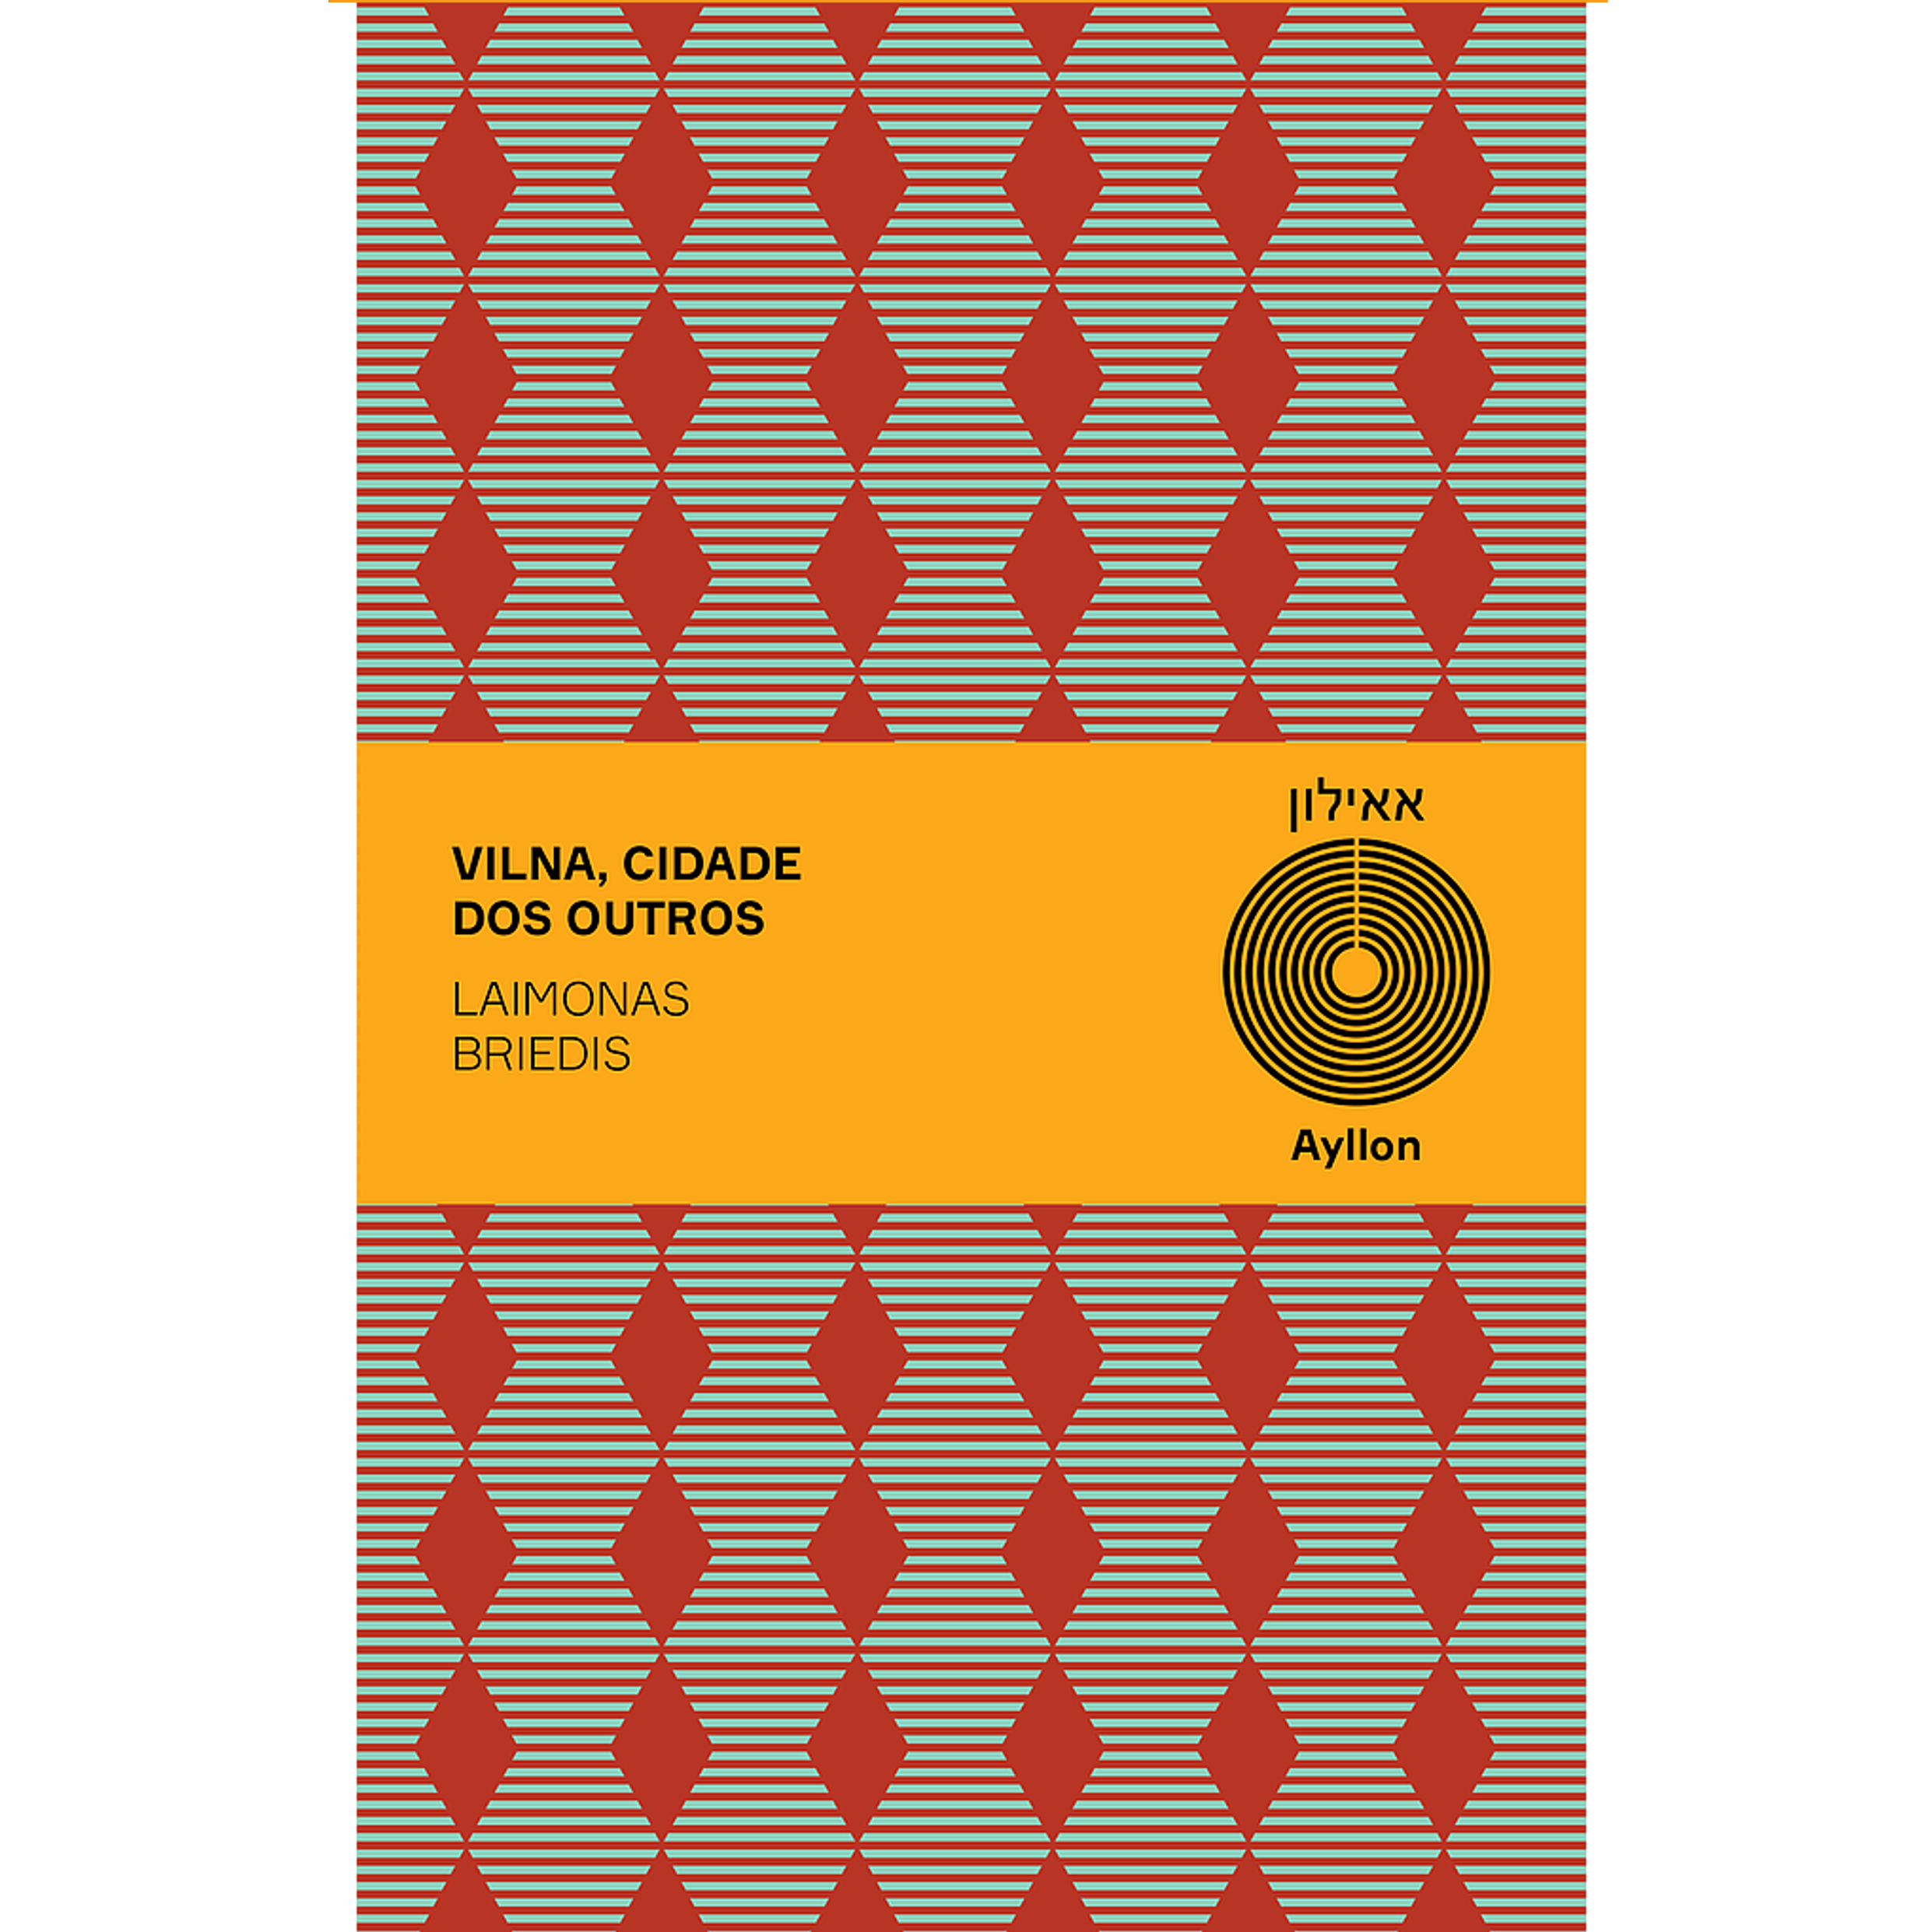
\includegraphics[width=74mm]{./CAPAS/vilna.jpg}
\end{center}
\hspace*{-7cm}\hrulefill\hspace*{-7cm}
\medskip

\noindent{}\textit{Vilna, cidade dos outros} é uma narrativa sobre a capital da Lituânia. \hlc{Escrita com base na cartografia histórica e geografia humana local, a cidade que também foi conhecida como "a Jerusalém da Lituânia" abrigou ao longo dos tempos inúmeros povos, falantes de diversos idiomas, em uma miscelânia cultural: judeus, poloneses, lituanos, ucranianos, bielorussos, russos, alemães, letões, armênios, tártaros e outros grupos minoritários}. Impregnada dentre seus vários componentes pelo barroco, que esteve no limiar da Europa e no contexto de suas mudanças, a cosmopolita cidade também é apresentada através de textos de pessoas ilustres ou desconhecidas, de muitas procedências e línguas, que viveram ou passaram por ela, através de relatos de experiências, sensibilidades e perspectivas próprias.

\vfill
\hspace*{-.4cm}\begin{minipage}[c]{1\linewidth}
\small\textbf{
\hspace*{-.1cm}Editora: Ayllon\\
Título: Vilna, cidade dos outros\\
Autor: Laimonas Briedis\\ 
ISBN: 978-85-77156-65-8\\
Páginas: 380\\
Formato: 13,3x21\,cm\\
Preço: R\$ 99,00
}
\end{minipage}
\pagebreak

\begin{center}
\hspace*{.5cm}
\includegraphics[width=74mm]{./CAPAS/breve.jpeg}
\end{center}
\hspace*{-7cm}\hrulefill\hspace*{-7cm}
\medskip

\noindent{}\textit{Acontecimentos na irrealidade imediata} foi originalmente publicado em 1936, e é composto por um amálgama caleidoscópico de situações que cruzam o caminho do narrador, um personagem desajustado ao mundo. Esses􏰃􏰀 acontecimentos arrastam-no a um turbilhão de pensamentos e ações atravessados por forças contrapostas, no qual as percepções misturadas da realidade, do tempo e do espaço dão lugar a um tipo diferente de discurso, que oferece inquietações fragmentadas ao invés de uma ordem racional.

\vfill
\noindent\begin{minipage}[c]{1\linewidth}
{\small\textbf{
\hspace*{-.1cm}Editora: Ayllon\\
Título: Acontecimentos na irrealidade imediata\\
Autor: Max Blecher\\ 
ISBN: 978-65-89705-07-9\\
Páginas: 170\\
Formato: 13,3x21\,cm\\
Preço: R\$ 54,00\\
}}
\end{minipage}
\pagebreak

\begin{center}
\hspace*{.5cm}
\includegraphics[width=74mm]{./CAPAS/breve.jpeg}
\end{center}
\hspace*{-7cm}\hrulefill\hspace*{-7cm}
\medskip

\noindent{}\textit{Em busca de meus irmãos na América}, de Chaim Novodvorsky, é um texto de memória que prende o leitor do começo ao fim. É um relato pessoal, singular, e, ao mesmo tempo, emblemático dos percursos da imigração judaica. Mescla de forma saborosa os acontecimentos e as aventuras pessoais de um imigrante polonês que foi primeiro à Argentina, depois ao Uruguai e, finalmente, ao Brasil, com um preciso e vívido retrato dos caminhos pelos quais se dava a inserção dos imigrantes na vida do país entre os anos 1920 e 1960. 

\vfill
\noindent\begin{minipage}[c]{1\linewidth}
{\small\textbf{
\hspace*{-.1cm}Editora: Ayllon\\
Título: Em busca de meus irmãos na América\\
Autor: Chaim Novodvorsky\\ 
ISBN: 978-65-89705-29-1\\
Páginas: 99 (provisório)\\
Formato: 13,3x21\,cm\\
Preço: R\$ 43,00\\
}}
\end{minipage}
\pagebreak

\vspace*{1.5cm}
\noindent{}{\nohyphens{\LARGE{Cacilds vidis litro abertis}}}
\bigskip

\hfill{}\scalebox{.8}{MUSSUM IPSUM}
\bigskip
\bigskip
\bigskip

\begin{multicols}{2}
\noindent{}\lipsum[2]
\lipsum[4]
\lipsum[6]

{\small\fakereceipt{
\noindent{}\lipsum[7]
}}
\vspace{\baselineskip}

\lipsum[2]
\lipsum[4]
\lipsum[6]

\noindent{}\textcolor{gray}{\footnotesize\slsc{Trecho de  “O livro dos mandamentos”.}}
\end{multicols}
